\documentclass{article}

% Recommended, but optional, packages for figures and better typesetting:
\usepackage{microtype}
\usepackage{graphicx}
\usepackage{subfigure}
\usepackage{booktabs} % for professional tables

\usepackage{hyperref}
\usepackage{amsmath}
\usepackage{amssymb}

\newcommand{\theHalgorithm}{\arabic{algorithm}}

\usepackage[accepted]{icml2018}

\icmltitlerunning{Online Recommendation via Particle Thompson Sampling}

\begin{document}

\twocolumn[
\icmltitle{Online Recommendation via Particle Thompson Sampling}
\begin{icmlauthorlist}
\icmlauthor{Michael Alvarino}{equal}
\icmlauthor{Bharat Srikishan}{equal}
\icmlauthor{Colby Wise}{equal}
\end{icmlauthorlist}
\icmlaffiliation{equal}{Columbia University}
\vskip 0.3in
]

\begin{abstract}
    Within the field of recommender systems various forms of collaborative filtering are often used to estimate how users will rate items. One of the most popular methods used when contextual information is not available is Probabilistic Matrix Factorization (PMF). This core method is capable of scaling with a large number of observations and performs well even when restricted to sparse datasets. Unfortunately PMF is limited to offline predictions for a fixed set of users and items. First, we present a fast online recommendation system using PMF, Thompson sampling, and particle filtering to provide cold start movie recommendations to users. Then we examine the effect of different particle sampling methods on particle degeneracy. Lastly, we provide a method for evaluating algorithm performance on users with high drift in preferences.
\end{abstract}

\section{Introduction}
PMF is the most common collaborative filtering method for recommendation systems. While it does provide useful recommendations for users it also requires a-priori knowledge of the set of users and items. Real world use cases must provide recommendations for users that have no previous history (cold start users). 

Online learning methods are designed to accept new users or items over time without sacrificing the efficiency or accuracy of the algorithm. In Efficient Thompson Sampling for Online Matrix Factorization Recommendation \cite{kawale2015efficient} (ETSOMF) an online algorithm is proposed, but is subject to a common problem in particle filtering methods: degeneracy.

A particle filtering algorithm is said be degenerate when, after only a few iterations, all but one particle has negligible weights. We propose several different particle resampling methods which combat the degeneracy problem and compare their performance on the MovieLens 100k Dataset.

\section{Model}

\subsection{Probabilistic Matrix Factorization}
Offline PMF computes a low rank factorization of a ratings matrix $R$ where $R = UV^\top$ for $U \in \mathbb{R}^{n \times k}$
and $V \in \mathbb{R}^{m \times k}$. $U$ and $V$ are user and item latent matrices and $K$ is small, for most of our experiments $K$ was less than $10$.

The PMF model assigns a Normal prior with zero mean and $K$ dimensional user-specific variance, $\sigma_u^2 I_K$, to the user latent matrix $U$ and a similar distribution to the item latent matrix $V$. Each rating $r_{i,j}$ is then assigned a Normal distribution centered on $U_iV_j^T$ with rating variance $\sigma^2$.

\begin{gather*}
U_i \sim \mathcal{N}(0, \sigma_u^2 I_K) \\
V_i \sim \mathcal{N}(0, \sigma_v^2 I_K) \\
r_{ij} | U, V \sim \mathcal{N}(U_i^\top V_j, \sigma^2)
\end{gather*}

This linear Gaussian model has an analytically solvable conditional posterior, but in order to support online inference we use a particle filtering method as described in ETSOMF.

\subsection{Particle Filtering}
Particle Filtering is a well known Sequential Monte Carlo method for performing inference where the system evolves over time based on information from noisy measurements. Sequential importance sampling ($SIS$) is a approximate Monte Carlo particle filtering method for analytically intractable systems. The goal of SIS is to approximate a posterior distribution with a weighted set of "samples" known as particles. The key idea is to update particles and their weights with new information at each step to better approximate the target posterior.  

Let $\{X_{0:k}^i, w_k^i\}_1^N$ denote N random measures representative of the posterior of a system, $p(x_{0:k}| z_{1:k})$. Then, we can approximate the true posterior of this system by the following:

\begin{gather*}
    p(x_{0:k}| z_{1:k}) \approx \Sigma_{i=1}^{N}w^i_k \delta(x_{0:k} - x^i_{0:k}) \\
    \text{where } \Sigma_i w_k^i = 1
\end{gather*}

Then, using sequential importance sampling, we can derive update equations for the weight associated with each particle as described in \cite{arulampalam2002tutorial}.

\subsection{Resampling}
A common problem with particle filtering methods such as SIS is particle $degeneracy$. Particle degeneracy is the tendency for only a few particle weights to have significant mass while all other weights drift toward zero as particles are successively updated.

Resampling is a common way to deal with the degeneracy problem. During resampling we draw a new set of N particles with replacement from the current particles based on the normalized weights of the current particle set. The advantage of this method is that it allows us to carry forward particles with high probability mass areas. The down-side of resampling is called $sample$ $impoverishment$. Sample impoverishment is when particles with large weights are sampled more frequently than low weight particles leading to a decrease in diversity of particles. It is common for the number of particles to collapse into a single particle which can negatively effect the quality of the approximation.

The original authors of ETSOMF saw degeneracy as a significant problem while training their algorithm. Our contribution is the analysis of new resampling methods for combating degeneracy. Specifically, we examine three primary resampling techniques, multinomial, stratified, and systematic resampling.

\subsubsection{Multinomial Resampling}
In multinomial resampling the particles are sampled from a multinomial distribution whose parameters are directly defined by the normalized, updated, weights of each particle \cite{douc2005comparison}.

\subsubsection{Stratified Resampling}
Stratified resampling breaks the interval into $n$ disjoint sets $(0, 1/n], ... , (\{n - 1\} / n, 1]$ and draws independently from the uniform distribution $U((\{i - 1\}/n, i/n])$ where $i$ is the $i$-ith sample \cite{douc2005comparison}.

\subsubsection{Systematic Resampling}
Systematic resampling deterministically links variables drawn in sub-intervals during stratified sampling. It does so by setting $U^i = (i-1)/n + U$, where $U$ is drawn from $U((0, 1/n])$.

$U$s generated via systematic resampling are known within the particle sampling literature as empirically good and computationally simple \cite{douc2005comparison}

\subsection{Particle Thompson Sampling}
We take advantage of the graphical structure of our probabilistic model to derive an efficient Rao-Blackwellized particle filter which maintains an estimate of the posterior over time. Additionally, we use Thompson sampling to choose particles and balance exploration with exploitation of our current posterior estimate.

Each particle stores parameters $U, V, \sigma_U, \sigma_V$ and for every update we sample $U_{i_t}|V, \sigma_U$
followed by $V_{j_t}|U, \sigma_v$ like so:
\begin{gather*}
P(U_i | V, R^o, \sigma, \sigma_U) = P(U_i | V_{rts(i)}, R^o_{i, rts(i)}, \sigma_U, \sigma) \\
= \mathcal{N}(U_i | \mu^u_i, (\Lambda_i^u)^{-1}) \\
\text{where } \mu_i^u = \frac{1}{\sigma^2}(\Lambda_i^u)^{-1})\zeta_i^u \\
\Lambda_i^u = \frac{1}{\sigma^2} \sum_{j \in rts(i)} V_j V_j^{\top} + \frac{1}{\sigma_u^2}I_K \\
\zeta_i^u = \sum_{j \in rts(i)} r_{ij}^o V_j
\end{gather*}


Here $R^o$ are the observed ratings and $rts(i)$ is the set of items rated by user $i$. The update for our sample of $V_j$ mirrors this update.


\section{Experiments}

\subsection{Data}
We ran our experiments on the MovieLens 100k dataset. We only used the rating data for our
online recommendations, however we used the genre data in our evaluation of user preference
drift. We subtracted the mean rating from the data to center ratings at 0.

This dataset has 943 users, 1683 movies, and 100,000 ratings.
\subsection{Latent Features vs Number of Particles}

\begin{table}[ht]
\caption{Mean squared error statistics on the test set for various choices of K
(latent dimensionality) and P (number of particles)}
\label{sample-table}
\vskip 0.15in
\begin{center}
\begin{small}
\begin{sc}
\begin{tabular}{lcccc}
\toprule
(K, P) & Mean & Std Dev & Min & Max \\
\midrule
(2, 2)  & 1.539 & 0.227 & 1.294 & 1.861 \\
(2, 5)  & 1.368 & 0.059 & 1.283 & 1.454 \\
(3, 5)  & 1.898 & 0.115 & 1.751 & 2.095 \\
(3, 10) & 1.818 & 0.085 & 1.742 & 1.964 \\
(3, 20) & 1.865 & 0.105 & 1.773 & 2.012 \\
(5, 10) & 2.648 & 0.076 & 2.537 & 2.774 \\
(5, 20) & 2.523 & 0.144 & 2.255 & 2.688 \\
\bottomrule
\end{tabular}
\end{sc}
\end{small}
\end{center}
\vskip -0.1in
\end{table}

The number of latent features (K) and number of particles (P) are two common hyperparameters. To empirically test how the number of latent features vs particle numbers effects performance, we run the algorithm five times for each (K, P) pair then compute the mean mean squared error, standard deviation, minimum and maximum value. From the results we select K=2 and P=5 given the pair has the lowest MSE and standard deviation.

Furthermore, we found the number of latent features to be the most significant hyperparameter for model performance as show in the table: increasing K lead to poorer performance. The number of particles is harder to explain. Somewhat counter intuitively we found that a lower number of particles leads to better results. The reason behind this may be that for this dataset most users reward preference can be approximated by 2-5 particles but more work in this area is needed.

\subsection{Particle Resampling Methods}

As discussed above, a common problem with particle filtering methods is degeneracy and sample impoverishment. To get a better sense for how these two common problems effected the algorithm we analyzed how the number of unique particles changed over time using three resampling methods: multinomial, stratified, and systematic resampling. Additionally, we compare mean squared errors for each method. 

Figure 1 below shows MSE results for each method which show that systematic resampling achieves the best MSE result followed by multinomial and stratified which are essentially equal. Systematic resampling showed the best result, similar to empirical results in other research \cite{doucet2009tutorial}.

\begin{figure}[ht]
\begin{center}
\centerline{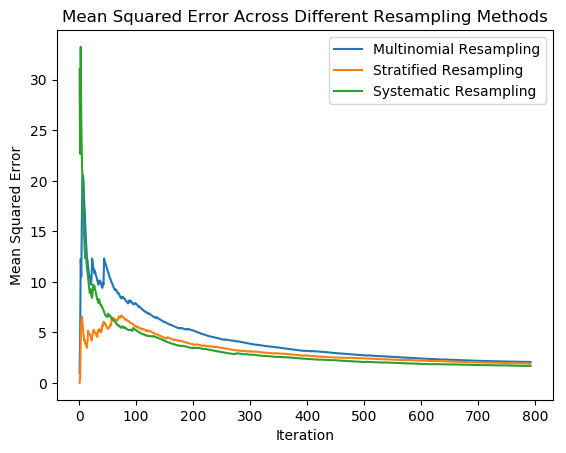
\includegraphics[width=\columnwidth]{mse_resample}}
\caption{MSE vs Resampling Method for K=2 and P=5}
\label{MSEResampling}
\end{center}
\vskip -0.4in
\end{figure}

\begin{figure}[ht]
\begin{center}
\centerline{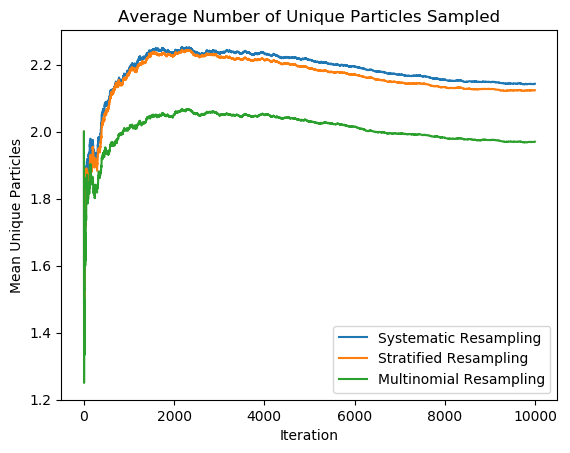
\includegraphics[width=\columnwidth]{num_unique_particles_when_resampling_k=2_np=10.png}}
\caption{MSE vs Resampling Method for K=2 and P=5}
\label{MSEResampling}
\end{center}
\vskip -0.4in
\end{figure}

Figure 2 shows the number of unique particles per iteration of the algorithm for each sampling method. The data was truncated at 10000 iterations because after this point the mean unique particles sampled all decreased linearly, in unison. The plot shows that on average, systematic resampling uses more unique particles at each iteration. 

\section{Results}

\subsection{Model Evaluation}

The final mean squared error using five particles and 2 latent features is 1.36. Moreover, the best Cumulative Take Rate achieved was .28.

\begin{figure}[ht]
\begin{center}
\centerline{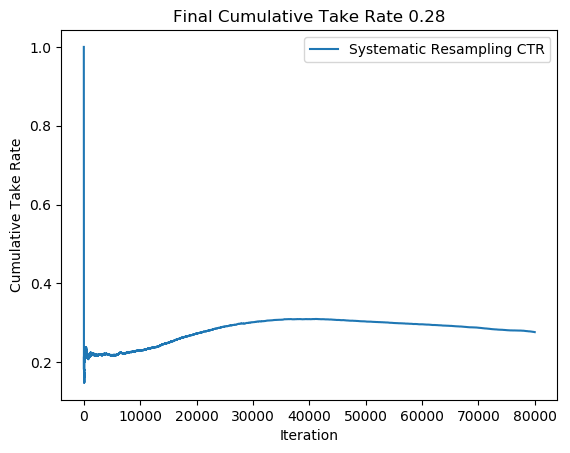
\includegraphics[width=\columnwidth]{CTR}}
\caption{Cumulative Take Rate}
\label{MSEResampling}
\end{center}
\vskip -0.4in
\end{figure}


\subsection{Cold Start Performance}
To test the performance of the algorithm on cold start users we randomly select 200 users who have viewed at least 120 movies. Then we learn the parameters of item features $V$ without the cold start users’ ratings similar to the approach taken in \cite{zhao2013interactive}. From here, we run the algorithm using the learned $V$ with the cold start users. Finally we take a snapshot of the precision of our algorithm at time intervals T=10, 20, 40, 120 and compare versus a baseline of randomly recommending items. As shown in Table 2, our algorithm outperforms the random baseline on cold start users at each time step.

\begin{center}
$precision@T$ = $\frac{1}{\#users}\sum\limits_{users}\sum\limits_{T=1}^{T}\theta hit$
\end{center}

\begin{table}[ht]
\caption{Cold Start Performance}
\label{sample-table}
\vskip 0.15in
\begin{center}
\begin{small}
\begin{sc}
\begin{tabular}{lccccc}
\toprule
Measure & \multicolumn{4}{c}{Precision}\\
Time Step  & 10     & 20     & 40   & 80    & 120 \\
\midrule
Random  &  0.020 & 0.045 & 0.065 & 0.130 & 0.165 \\
PTS     &  0.055 & 0.090 & 0.180 & 0.285 & 0.450 \\
\bottomrule
\end{tabular}
\end{sc}
\end{small}
\end{center}
\vskip -0.1in
\end{table}

\subsection{User Preference Drift}

Capturing user preference drift in online recommendation engines is difficult and we know of no standard methodology for capturing drift. In this paper we present one possible method that is intuitive and easy to explain. Similar to the cold start user experiment, our goal here is examine how the algorithm performs on users that display significant preference drift over time.  

To identify users with high drift over time, we randomly select 200 users with greater than 120 rated items. Next, each user's rating history is sorted by time stamp. We chosen to analyze drift at two distinct time stamps $T=60$ and $T=120$ where $T$ represents the number of rated items at step $T$. Using the two subsets of items for each user, we get the genre information for each item. There are 19 genres in the MovieLens 100k dataset including one unknown. For each item we get the binary representation of the genre where movies can have multiple genres describing them i.e. 'Action' and 'War'. For each user and time bucket a vector representing their genre distribution is obtained from their rated items history.

\begin{center}
cosine similarity $\theta = \frac{a \dot b}{||a|| \dot ||b||}$ \\
\ \newline
a = $user_i$ genre distribution @T=60 \\
b = $user_i$ genre distribution @T=120 \\
\end{center}

The chosen distance metric we use is cosine similarity where we choose the top 5 users with lowest cosine similarity from $T=60$ to $T=120$. We make no claims at to the optimality of this method for capturing drift, however we found it intuitive to explain and analyze. 

\begin{figure}[ht]

\begin{center}
\centerline{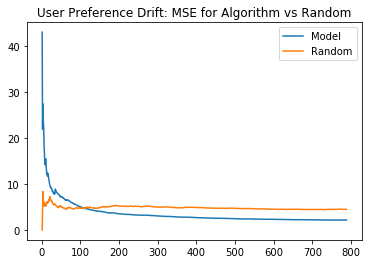
\includegraphics[width=\columnwidth]{drift_MSE}}
\caption{High drift user set mean squared error of our model vs random ratings with K = 2 and 5 particles.}
\label{drift_MSE}
\end{center}

\vskip -0.2in
\end{figure}

\begin{figure}[ht]

\begin{center}
\centerline{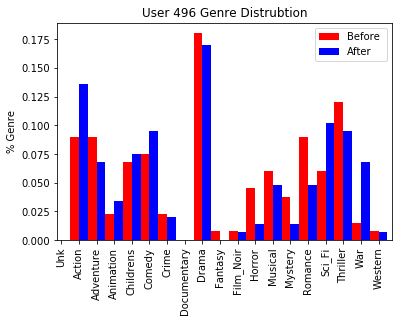
\includegraphics[width=\columnwidth]{drift_histogram}}
\caption{Visualization of genre drift for User 496 between "Before" (first 60 time steps) and "After" (last 60 time steps).}
\label{drift_histogram}
\end{center}

\vskip -0.2in
\end{figure}

We present user $496$ as a case study. User 496 displayed high preference drift as defined above. Qualitatively we can see that by time step 120 their genre distribution changed in the following way: war movies increased 5\% and romance decreased 4\% while action and Sci-Fi increased 4\% in their genre distribution. The MSE graph (Figure 4) for similar high drift users shows that the aggregate algorithm performance outperformed baseline random selection.  

\section{Conclusion and Future Work}

\nocite{kawale2015efficient}
\nocite{wang2017online}
\nocite{zhao2013interactive}
\nocite{cherkassky2013sequential}
\nocite{arulampalam2002tutorial}
\nocite{douc2005comparison}
\nocite{doucet2009tutorial}
\nocite{orhan2012particle}
\nocite{lo2017temporal}
\nocite{lindsten2015rao}

\bibliographystyle{icml2018}
\bibliography{report}

\end{document}
